\chapter[Medidas de Satisfação]{Medidas de Satisfação}
\section{Tecnicas de Interação Humano-Computador}
No design de interface de usuário deve ser considerado fatores que facilite a utilização da aplicação, além de ser atraente para o usuário. Para isso é necessário aplicar técnicas das quais é possível medir a eficiência, eficacia e satisfação do usuário. Isso é chamado de usabilidades.

As medidas de usabilidade podem ser obtidas por:

\begin{itemize}
	\item Medidas objetivas: está relacionada ao desempenho do usuário enquanto usa a interface. Promovem dados de tempo, velocidade ou ocorrencia de eventos particulares.
	\item Medidas subjetivas: representam a opnião do usuário para com a interface. São dados de sentimentos, atitudes, preferência.
\end{itemize}

\section{Técnica de Questionamento}

A técnica de questionamento identifica se os requisitos estão de acordo com a necessidade do usuaŕio. Uma técnica simples e barata de administrar e demonstram resultados significativos que podem mostrar necessidades que o designer não havia considerado.
Há dois modos de aplicar um questionamento: entrevista e questionários.

\section{Questionário}

 A vantagem do questionário em cima da entrevista, é que pode ser aplicado em um grande número de pessoas, além de apresentar dados quantitativos. É possível utilizar o questionário em várias fases do processo de design.
 Os questionários devem ser bem elaborados, compreensíveis e que gerem resultados que são adequados para a análise.

 \section{Coleta dos Dados}

 Avaliar subjetivamente com um questionário é umportante para a avaliação de usabilidade. Por isso foram elaborados modelos de questionários para essa finalidade. Os mais conhecidos são:

 \begin{itemize}
	\item QUIS (Questionnaire for User Interaction Satisfaction);
	\item SUMI (Software Usability Measurement Inventory);
	\item WAMMI (Website Analysis and MeasurMent Inventory)
	\item SUS (System Usability Scale).
\end{itemize}

\subsection{QUIS}
Desenvolvido por uma equipe multidisciplinar de pesquisadores do HCIL (Human-Computer Interaction Laboratory) da University of Maryland. Pode ser configurada de acordo com a necessidade de análise de cada interface. Dividido em seções onde cada uma especifica algum ponto de interesse da interface.
As questões são feitas em forma de afirmações e utilizam uma escala diferencial semântica, de 0 a 9, onde zero apresenta o total negativo e 9 o total positivo.

\begin{figure}[h]
	\centering
	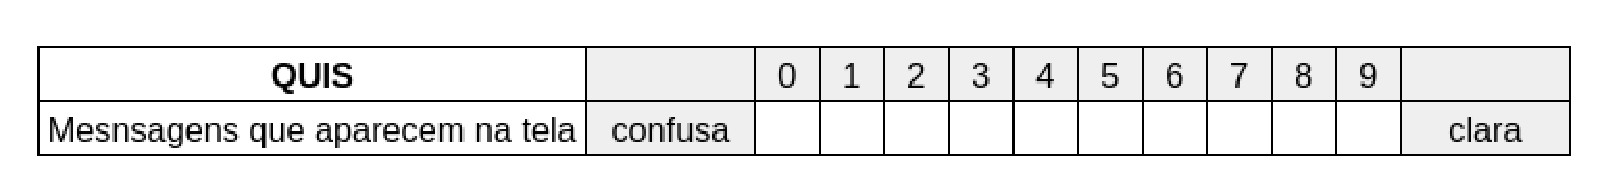
\includegraphics[scale=0.5]{figuras/quis.eps}
	\caption{Exemplo de questão no modelo QUIS}
\end{figure}

Uma vantagem da utilização do QUIS é que se trata de um modelo amplamente utilizado em vários ciclos de qualificação e centenas de estudos. Portanto, é um modelo consistente.

\subsection{SUMI}
Desenvolvido pelo HFC (Human Factors Group) da University College. Pode encontrar falhas de usabilidade e mostrar uma visão do usuário final. Consiste em 50 questões de afirmações escalares em três níveis: "concordo", "não sei" e "não concordo", como mostra a figura abaixo.

\begin{figure}[h]
	\centering
	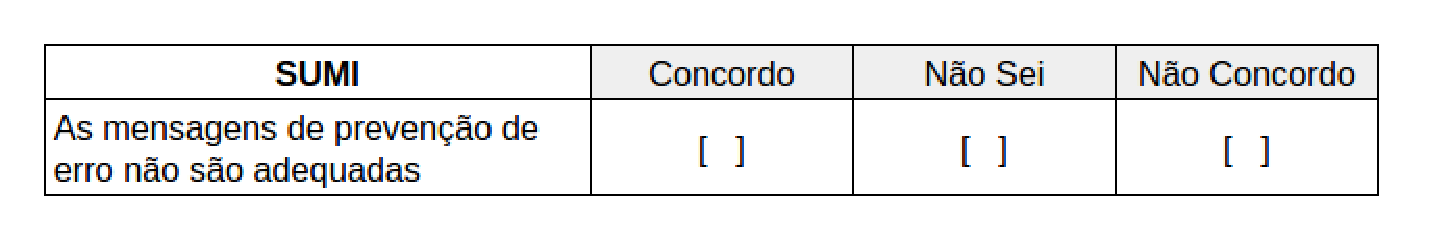
\includegraphics[scale=0.5]{figuras/sumi.eps}
	\caption{Exemplo de questão no modelo SUMI}
\end{figure}

\subsection{WAMMI}
O serviço WAMMI iniciou em 1996 para análise de Websites, exclusivamente. É utilizado para avaliar os seguintes aspectos: atratividade, controle, eficiência, utilidade, aprendizagem e usabilidade global. O serviço conta com um questionário contendo 20 afirmações e uma única base de dados internacional. Um relatório é gerado ao final de um período de avaliação, que inclui:
\begin{itemize}
	\item Uma medida objetiva das reações do usuário para seu Website;
	\item Perfil do usuário WAMMI;
	\item Um mapeamento da análise do visitante incluindo as principais razões pelas quais o usuários visitam seu site;
	\item Uma análise de melhoria do site;
	\item Uma análise estatística e tabulações cruzadas;
	\item Dados numéricos para análises posteriores;
\end{itemize}

\subsection{SUS}
Desenvolvido como parte do programa de engenharia de usabilidade integrado a Digital Equipment Co Ltd. Consiste em um questionário com 10 afirmações no formato de escala Likert, que mede o grau de concordância em uma escala de cinco pontos, como mostra a figura abaixo.

\begin{figure}[h]
	\centering
	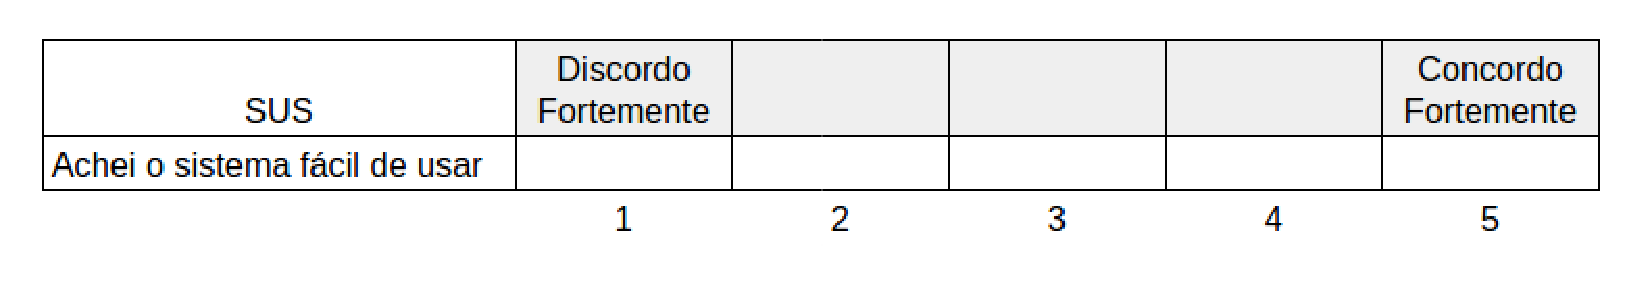
\includegraphics[scale=0.5]{figuras/sus.eps}
	\caption{Exemplo de questão no modelo SUS (escala Likert)}
\end{figure}

O SUS é distribuido gratuitamente e se mostra robusta e confiável, provendo um alto nível de subjetividade.

\nocite{FILARDI_TRAINA_2008}

\section{Utilização dos Questionário no Processo de Avaliação}

Durante o processo de avaliação será utilizado dois tipos de questionários: pré-sessão e pós-sessão.
\begin{itemize}
	\item O questionário pré-sessão será utilizado para coletar dados sobre o perfil do usuário da aplicação abordando alguns aspectos do seu comportamento. É composto por questões fechadas e questões abertas.
	\item O questionário pós-sessão será usado para obter feedback sobre a experiencia de utilização da aplicação.
\end{itemize}

\begin{figure}[h]
	\centering
	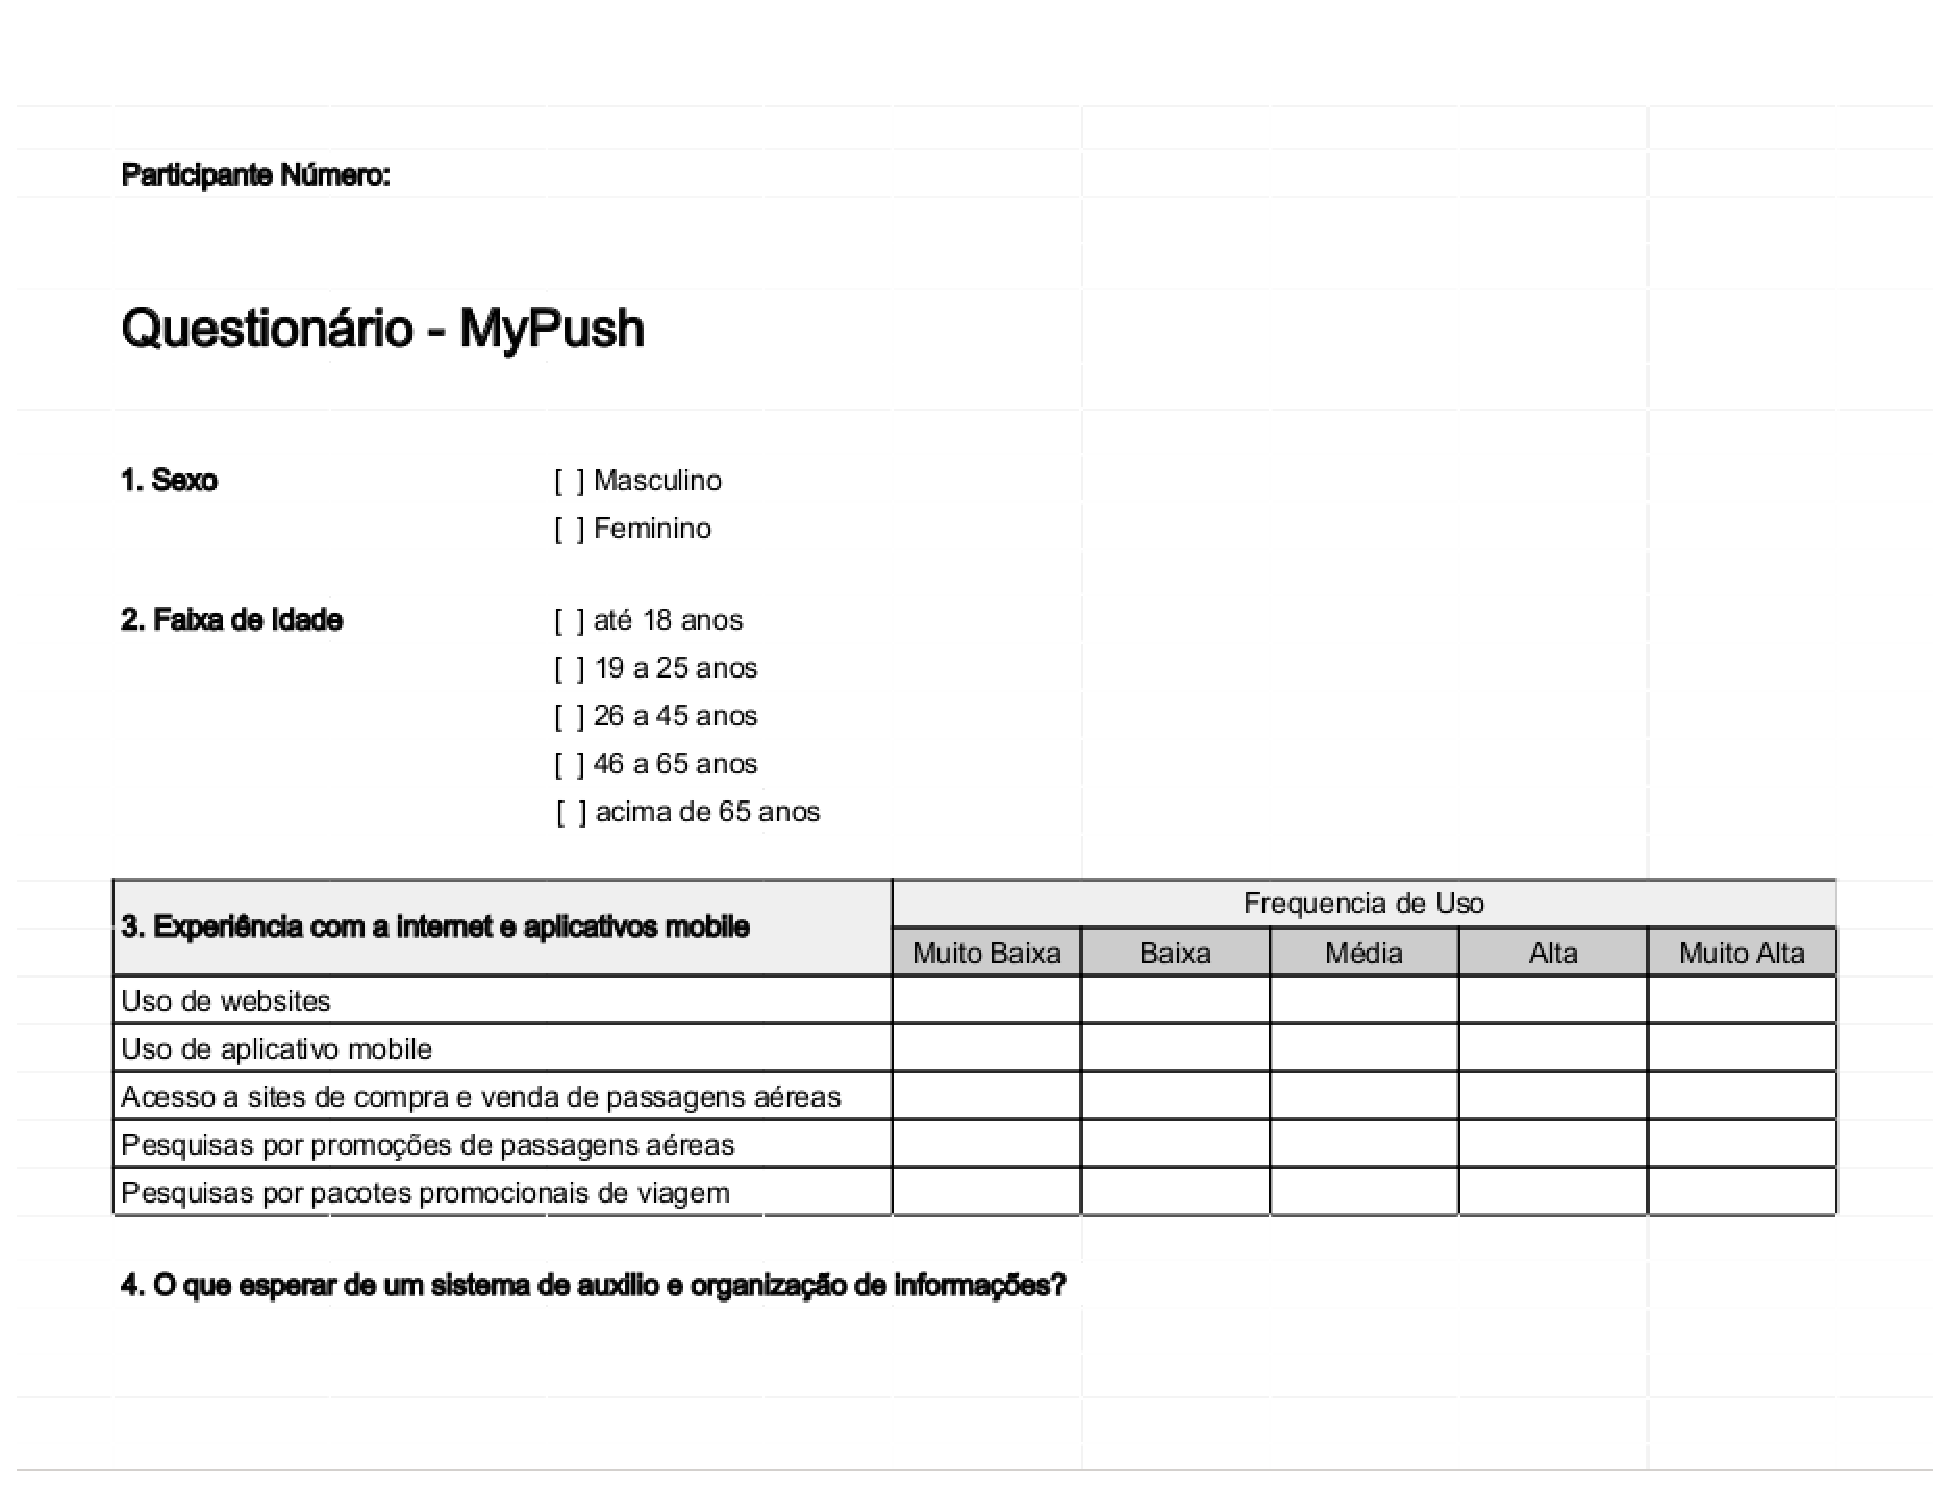
\includegraphics[scale=0.5]{figuras/questionario_pre-sessao.eps}
	\caption{Questionário pré-sessão}
\end{figure}
